% !Tex root = main.tex
\newpage
\section{Discussion}
The purpose of the experiments conducted in this work is to demonstrate the applicability of learned models for dependency detection.
In the following paragraphs, the results of the experiments are discussed in this context.

\subsection{Robustness}
Robustness is introduced as a measure of the imputation-capabilities of a FD using FD Imputer.
It is successfully demonstrated that FDs with a high robustness also contain humanly explainable meanings, for example when discussing figure~\ref{fig:f1_fd_adult}.

In the field of data profiling, it was proposed that ``any dependency [could] be turned into a rule to check for errors in the data''.\cite[p.~9]{ABE19}
This does not seem to be the case in general, but only for highly robust FDs with classfiable values in the RHS.

If a FD countains sequential values in the RHS, FD Imputer generally performs poorly.
As shown in table~\ref{tab:fd-imputer-mse}, FD Imputer does not retrieve imputations for most RHSs in the test-set.
In future works, implementing FD Imputer with a selection of RFDs might lead to further insights regarding robustness of dependencies containing sequential RHS values.

\subsection{Comparing ML Imputer with FD Imputer}
FD Imputer is implemented to probe the feasibility of value imputation using FDs.
The usage of FDs for value implementation also makes a comparison with learned classifiers and regression-models possible.

The behavior of FD Imputer is similar to what can be observed when analyzing a case of overfitting.~\cite[p.~56]{SMO08}
Haykins writes that ``[Overfitting] is essentially a `look-up table', which implies that the input-output mapping [\dots] is not smooth.''~\cite[p.~165]{HAY08}
The way FD Imputer functions is \emph{literally} by using the test-set as a look-up table.

\subsubsection{Imputing Sequential RHSs}
Since FDs are established by exact equality of values, imputations of sequential values are very rare and, if they exist, either extremely accurate or very wrong (see table~\ref{tab:fd-imputer-mse-abalone}.
FD Imputer cannot approximate numerical values, due to the definition of a FD.
Data is always assumed to be classifiable.

In contrast to this, ML-Imputer is able to perform regression, predicting a continuous label for a given input with a specific uncertainty.
This circumstance leads to a far superior performance of ML Imputer when imputing continuous values.
Although MSEs for the FD Imputer model are generally smaller than MSEs measured for models trained with DepDetector, this effect is just a manifestation of the overfitting that takes place when FD Imputer looks up values.
This result is emphasized by the findings in table~\ref{tab:fd-imputer-mse}:
On the datasets considered in this work, FD Imputer cannot retrieve imputations from the test-set for an average of 99.8\% of RHS values.

\subsubsection{Imputing Classifiable RHSs}
Figure~\ref{fig:f1_ml_fd_adult} compares the F1-Scores of both ML Imputer and FD Imputer on the Adult dataset.
One can observe that for almost all FDs, ML Imputer performs better than the FD Imputer.
FD Imputer performance and ML Imputer performance appear to be partially proportional.
If the score achieved by ML Imputer is lower than 0.7, the FD Imputer's F1-Score for the same FD is 0.
\begin{figure}[ht]
     \centering
     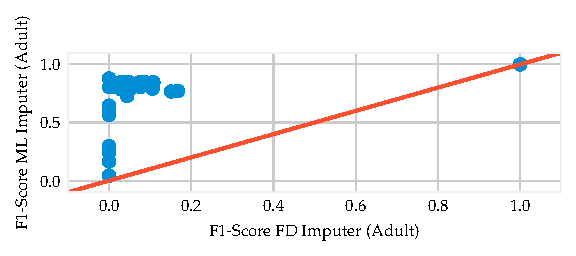
\includegraphics[width=\textwidth]{../figures/adult/f1_ml_fd}
     \caption{The figure compares the F1-Score of the FD Imputer compared to the F1-Score of ML Imputer. Each point represents one FD.}
     \label{fig:f1_ml_fd_adult}
 \end{figure}

However, for FDs where ML Imputer's scores are bigger than 0.7, the FD Imputer's scores are bigger than 0.
The two FDs for which the FD Imputer performs as well as the ML Imputer were identified and discussed in the previous sections.

\subsubsection{Overfitting ML Imputer}
In order to mimic the overfitting that takes place when FD Imputer looks up imputations on the train-set, it might be interesting to overfit ML Imputer models on purpose.
As shown in figure~\ref{fig:f1-ml-overfit-adult} and figure~\ref{fig:mse-ml-overfit-fractions}, neither the classifier-models, nor the regression-models trained by ML Imputer are capable of overfitting.
Future research-effort could be put into overfitting the models trained by ML Imputer with the goal of approximating the properties of FD Imputer.

\subsection{Dependency Detection with DepDetector}
- stupid implementation with trees
- complete super slow
- might be interesting to reduce compute time since dependencies are searched by solving a minimization problem on a graph

\section{Conclusion}
The experiments conducted in the previous section explored the characteristics of FDs.
When applied for database scheme normalization, FDs serve a well-defined purpose.
However, when it comes to obtaining insights about non-static data, FDs seem to provide little insights about what to expect from new rows that might be added in the future.

FDs do not seem fit for obtaining human-readable information about a (relational) database that is being used in a deployed application.
FDs show no resistance to noisy data due to the static nature of their definition.
